\documentclass[10pt]{article}
\usepackage{amsmath}
\usepackage{mathtools}
\DeclarePairedDelimiter\ceil{\lceil}{\rceil}
\usepackage{mathptmx}
\DeclarePairedDelimiter{\abs}{\lvert}{\rvert}
\usepackage[hidelinks]{hyperref}
\usepackage{amssymb}
\usepackage{tikz}
\usepackage{caption}
\usepackage{graphicx}
\usepackage[T1]{fontenc}
\graphicspath{{.}}
\usepackage{listings}
\usepackage{verbatim}
\lstset{
language=[LaTeX]TeX,
backgroundcolor=\color{gray!25},
basicstyle=\ttfamily,
columns=flexible,
breaklines=true
}
\captionsetup{labelsep=space,justification=justified,singlelinecheck=off}
\reversemarginpar
\usepackage[paper=a4paper,
            %includefoot, % Uncomment to put page number above margin
            marginparwidth=20mm,      % Length of section titles
            marginparsep=0.8mm,       % Space between titles and text
            margin=12mm,              % 25mm margins
            includemp]{geometry}

\begin{document}
\section*{}
\begin{flushleft}
Name: Krishna Chaitanya Sripada\\
\end{flushleft}
\section*{Ans 2.3}
\begin{flushleft}
Since the set concepts are of the form c = \{(x,y): $x^{2} + y^{2} \leq r^{2}$\} , the circle is around the origin with radius r. Let us choose a smaller radius q such that both of them have the same center i.e., origin.\\
\vspace{0.5em}
Let A denote the region between circle with radius `r' and circle with radius 'q' such that A = $\{ x: q \leq \|x\| \leq r \}$. Let $P_{r}[A]$ denote the probability mass of the region defined by A, that is the probability that a point randomly drawn falls within A. Since errors made by the PAC-learning algorithm can be only due to points falling inside A, we can assume that $P_{r}[A] > \epsilon$ ; otherwise the error of A is less than or equal to $\epsilon$ regardless of the training sample.\\
\vspace{0.5em}
Let R$\in$c be a target concept and H be a hypothesis and by contraposition, if R(A) > $\epsilon$, then any point in H chosen accordingly will ``miss'' region A with a probability of at most 1 - $\epsilon$. Therefore, we get,\\
\vspace{0.5em}
$P_{r}[R(A) > \epsilon] \leq P_{r}[\{A \cap H = \varnothing \}]$\\
\hspace{1.8cm} $\leq {(1 - \epsilon)}^{m}$\\
\hspace{1.8cm} $\leq {e}^{-m\epsilon}$\\
where for the last step, the identity 1-x $\leq e^{-x}$ is used which is valid for all x $\in \mathbb{R}$.\\
\vspace{0.5em}
For any $\delta$ > 0, to ensure that $P_{r}[R(A) > \epsilon] \leq \delta$, we can impose,\\
\hspace{1.8cm} ${e}^{-m\epsilon} \leq \delta \Leftrightarrow$ m $\geq (1/\epsilon) \log (1/\delta)$
\end{flushleft}
\section*{Ans 2.4}
\begin{flushleft}
Given X = $\mathbb{R}^{2}$ and the set of concepts are of the form c = $\{x \in \mathbb{R}^{2}: \|x- x_{0}\| \leq r\}$ for some point $x_{0} \in \mathbb{R}^{2}$ and real number \textit{r}. Also the complexity is $m \geq (3/\epsilon) \log(3/\delta)$ with three regions $r_{1}, r_{2}, r_{3}$ drawn around the edge of concept \textit{c} have probability of $\epsilon/3$ each.\\
\vspace{0.5em}
Gertrude is relying on the implication that generalization $error > \epsilon \Rightarrow H \cap r_{i} = \varnothing$ for some \textit{i} and hypothesis \textit{H}. Below is the illustration of an example where we have one training point in each region. The points in $r_{1}$ and $r_{2}$ are very close together, and the point in $r_{3}$ is very close to region $r_{1}$. In this data, the learned circle includes these points and one diameter approximately traverses the corners of $r_{1}$. In the illustration below, the circle with the thick border is our target circle and the darkened areas are the errors of this hypothesis. Apparently, the error can be greater that $\epsilon$ even while $H \cap r_{i} = \varnothing$ $ \forall$ i and this invalidates Gertrude's proof.  
\begin{figure}[!htb]
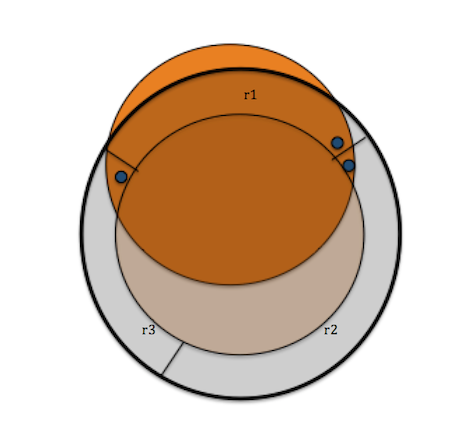
\includegraphics{Non-CC.png}
\caption{:Non-concentric circles}
\end{figure}
\end{flushleft}
\vspace{10em}
\section*{Ans 2.6}
\begin{flushleft}
(a) The probability that $R^{'}$ misses region $r_{j}$ is the product of the probability \textit{p} for each point $x_{i}$ of the training sample that \\
i. Doesn't fall in $r_{j}$ or be positive.\\
ii. Fall in $r_{j}$ with the label flipped to negative because of the noise.\\
Then, we have, \\
\hspace{2em} $p = P_{r}[x \not\in r_{j} \lor (x \in r_{j} \land $ \textit{x} is positive $\land$ label of \textit{x} is flipped$)]$\\
\hspace{2.8em} $= P_{r}[x \not\in r_{j} \lor (x \in r_{j} \land $ label of \textit{x} is flipped$)]$\\
\hspace{2.8em} $= P_{r}[x \not\in r_{j}] + P_{r}[(x \in r_{j} \land$ label of \textit{x} is flipped$)]$\\
\hspace{2.8em} $= (1 - P_{r}[x \in r_{j}]) + \eta P_{r}[x \in r_{j}]$\\
\hspace{2.8em} $= (1- \eta) (1- P_{r}[x \not\in r_{j}]) + \eta$\\
\hspace{2.8em} $\leq (1- \eta) (1- \epsilon/4) + \eta$ ( by the definition of PAC learnability)\\
\hspace{2.8em} $= (1- \epsilon/4) + \eta \epsilon/4$\\
\hspace{2.8em} $\leq 1- \epsilon(1 - \eta^{'})/4$\\
\vspace{0.5em}
(b) The probability that $P_{r}[R(R^{'})> \epsilon]$ is upper bound by the probability that $R^{'}$ misses at least one region $r_{j}$. Thus, by union bound, we get, \\
\hspace{2em} $P_{r}[R(R^{'}) > \epsilon ] \leq 4 (1- \epsilon(1 - \eta^{'})/4)^{m}$\\
\hspace{2em} $P_{r}[R(R^{'}) > \epsilon ] \leq 4 e^{-m \epsilon(1 - \eta^{'})/4}$\\
\vspace{0.5em}
By setting $\delta$ to match the upper bound will result in a probability of at least 1 - $\delta$, $m \geq \frac{4}{(1- \eta^{'}) \epsilon} \log \frac{4}{\delta}$ with $R(R^{'}) \leq \epsilon$ 
\end{flushleft}
\section*{Ans 3.5}
\begin{flushleft}
Consider the case where \textit{H} is reduced to the constant hypothesis $h_{1} : x \mapsto 1$ and $h_{-1}: x \mapsto -1$. Then by definition of Rademacher complexity, \\
\hspace{2em} $\hat{R_{s}}(H) = \frac{1}{m} E_{\sigma} [sup \{\sum\limits_{i =1}^{m} \sigma_{i}, \sum\limits_{i=1}^{m} - \sigma_{i} \}] = \frac{1}{m} E_{\sigma} [\abs{\sum\limits_{i=1}^{m} \sigma_{i}}]$\\
\vspace{0.5em}
Let $X = \sum\limits_{i=1}^{m} \sigma_{i}$. Since E[$X^{2}$] = $E[\sum\limits_{i,j=1}^{m} \sigma_{i} \sigma_{j}]$ and $\forall i\neq j$ and $\sigma_{i}$ and $\sigma_{j}$ are independent, we get $E[\sigma_{i} \sigma_{j}] = E[\sigma_{i}] E[\sigma_{j}] = 0$. Thus, \\
\vspace{0.5em}
\hspace{2em} $E[X^{2}] = E[\sum\limits_{i}^{m} \sigma_{i} \sigma_{i}] = E[\sum\limits_{i}^{m} \sigma_{i}^{2}]$.\\
Since $m = E[X^{2}]$, it can be rewritten as $E[\abs{X}^{\frac{2}{3}} \abs{X}^{\frac{4}{3}}] \leq E{[\abs{X}]}^{\frac{2}{3}} E{[X^{4}]}^{\frac{1}{3}}$.\\
\vspace{0.5em}
Therefore,\\
\hspace{2em} $E[\abs{X}] \geq \frac{m^{\frac{3}{2}}}{E{[X^{4}]}^{\frac{1}{2}}} = \frac{m^{\frac{3}{2}}}{\sqrt{E[\sum\limits_{i=1}^{m} \sigma_{i}^{4} + 3 \sum\limits_{i \neq j} \sigma_{i}^{2} \sigma_{j}^{2}]}} = \frac{m^{\frac{3}{2}}}{\sqrt{m + 3m(m-1)}} = \frac{m^{\frac{3}{2}}}{\sqrt{m(3m-2)}} \geq \frac{m^{\frac{3}{2}}}{\sqrt{m(3m)}} = \sqrt{\frac{m}{3}}$.\\
\vspace{0.5em}
Thus,\\
\hspace{2em} $\hat{R_{s}}(H) \geq \sqrt{\frac{m}{3}}$\\
\vspace{0.5em}
Since $R_{m}$(H) $\leq \hat{R_{s}}(H) + O(\frac{VCdim(H)}{\sqrt{m}})$, it implies $R_{m}$(H) $\leq O(\frac{VCdim(H)}{\sqrt{m}})$, which contradicts $R_{m}$(H) $\leq O(\frac{VCdim(H)}{m})$.
\end{flushleft}
\section*{Ans 3.6}
\begin{flushleft}
A sequence of $2k+1$ points on a line can't be shattered if successive points are labeled with alternate labels starting with a positive label. We need to choose intervals which contain a longest sequence of consecutive positive sample points and we can have at most $2k$ such intervals. Thus, VC dimension of the class of union of $k$ intervals on a real line is $2k$.
\end{flushleft}
\section*{Ans 3.12}
\begin{flushleft}
(a) For any x $\in \mathbb{R}$, let there exist an $\omega$ with labels $- - + -$. Then $\sin(\omega x) < 0$, $\sin(2 \omega x) < 0$, $\sin(3 \omega x) > 0$ and $\sin(4 \omega x) < 0$. If we show that this implies $\sin^2(\omega x) < \frac{1}{2}$ and $\sin^2(\omega x) \geq \frac{3}{4}$, then it will be a contradiction.\\
\vspace{0.5em}
Using the identity $\sin(2\theta) = 2 \sin(\theta) \cos(\theta)$ and since $\sin(4 \omega x) < 0$, we have,\\
\hspace{2em} $2\sin(2 \omega x) \cos(2 \omega x) = \sin(4 \omega x) < 0$.\\
\vspace{0.5em}
Since $\sin(2 \omega x) < 0$, we can divide both sides of the inequality by $2\sin(2 \omega x)$ to get $\cos(2\omega x) > 0$. Applying the identity $\cos(2\theta) = 1 - 2\sin^2(\theta)$ yields $1 - 2\sin^2(\omega x) > 0$, or $\sin^2(\omega x) < \frac{1}{2}$. \\
\vspace{0.5em}
 Using the identity $\sin(3\theta) = 3 \sin(\theta) - 4 \sin^3(\theta)$ and $\sin(3 \omega x) \geq 0$, we have\\
 \hspace{2em} $3 \sin(\omega x) - 4 \sin^3(\omega x) = \sin(3 \omega x) \geq 0 $.\\
 \vspace{0.5em}
 Since $\sin(\omega x) < 0$ we can divide both sides of the inequality by $\sin(\omega x)$ to get $3 - 4 \sin^2(\omega x) \leq 0$ or $\sin^2(\omega x) \geq \frac{3}{4}$. Hence we have proved the contraction and thus $\forall x \in \mathbb{R}$, the points $x, 2x, 3x$ and $4x$ cannot be shattered by this family of sine functions.\\
\vspace{0.5em}
(b) For any $m>0$, consider points $(x_{1}, x_{2},....., x_{m})$ with arbitrary labels $(y_{1}, y_{2},......, y_{m})$ $\in \{-1, +1\}^{m}$. Now, let parameter $\omega = \pi(1+ \sum\limits_{i=1}^{m} 2^{i} y_{i}^{'})$ where $y_{i}^{'} = \frac{1-y_{i}}{2}$. If we can show that this parameter will classify the entire sample for any $m>0$ and choice of labels, then we can show that the VC-dimension of the family of sine functions is infinite.\\
\vspace{0.5em}
$\forall \in [1,m]$, we have\\
\hspace{2em} $\omega x_{j} = \omega 2^{-j} = \pi(2^{-j} + \sum\limits_{i=1}^{m} 2^{i-j} y_{i}^{'})$\\
\hspace{7.5em}$= \pi(2^{-j} + (\sum\limits_{i=1}^{j-1} 2^{i-j} y_{i}^{'}) + y_{j}^{'} + (\sum\limits_{i=1}^{m-j} 2^{i} y_{i}^{'}))$\\
\vspace{0.5em}
The last term can be ignored as it only contributes multiples of $2\pi$. Since $y_{i}^{'} \in \{0,1\}$ the sum of remaining terms is, $\pi(2^{-j} + (\sum\limits_{i=1}^{j-1} 2^{i-j} y_{i}^{'}) + y_{j}^{'}) = \pi(\sum\limits_{i=1}^{j-1} 2^{-i}y_{i}^{'} + 2^{-j}+ y_{j}^{'})$\\
Now the upper and lower bounds are as follows:\\
\vspace{0.5em}
\hspace{2em}$\pi(\sum\limits_{i=1}^{j-1} 2^{-i}y_{i}^{'} + 2^{-j} + y_{j}^{'}) \leq \pi(\sum\limits_{i=1}^{j} 2^{-i} + y_{j}^{'}) < \pi(1+y_{j}^{'})$\\
\hspace{2em}$\pi(\sum\limits_{i=1}^{j-1} 2^{-i}y_{i}^{'} + 2^{-j} + y_{j}^{'}) > \pi y_{j}^{'}$\\
Thus, if $y_{j} = 1$ we have $y_{j}^{'} = 0$ and $0< \omega x_{j} < \pi$, which implies $\sin(\omega x_{j}) = 1$. Similarly, for $y_{j} = -1$ we have $\sin(\omega x_{j}) = -1$
\end{flushleft}
\section*{Ans 3.19}
\begin{flushleft}
(a) By definition of Oskar's prediction rule,\\
\vspace{0.5em}
\hspace{2em}$error(f_{o}) = P_{r}[f_{o}(S) \neq x]$\\
\hspace{5.7em} $= P_{r}[f_{o}(S) = x_{A} \land x = x_{B}] + P_{r}[f_{o}(S) = x_{B} \land x = x_{A}]$\\
\hspace{5.7em} $= P_{r}[N(S) < \frac{m}{2} \lvert x= x_{B}] P_{r}[x = x_{B}] + P_{r}[N(S) \geq \frac{m}{2} \lvert x = x_{A}] P_{r}[x = x_{A}]$\\
\hspace{5.7em} $= \frac{1}{2}P_{r}[N{S} < \frac{m}{2} \lvert x = x_{B}] + \frac{1}{2}P_{r}[N(S) \geq \frac{m}{2} \lvert x = x_{A}] \geq \frac{1}{2} P_{r}[N(S) \geq \frac{m}{2} \lvert x = x_{A}]$\\
\vspace{0.5em}
(b) Since $P_{r}[N(S) \geq \frac{m}{2} \lvert x = x_{A}] = P_{r}[B(m,p) \geq k],$ with $p = \frac{1-\epsilon}{2}, k = \frac{m}{2}$ and $mp \leq k \leq m(1-p)$. Thus, by the binomial inequality given in the appendix, \\
\hspace{2em} $error(f_{o}) \geq \frac{1}{2}P_{r}[N \geq \frac{\frac{m\epsilon}{2}}{\sqrt{\frac{1}{4(1- \epsilon^{2})m}}}] = \frac{1}{2} P_{r} [N \geq \epsilon \sqrt{\frac{m}{1 - \epsilon^{2}}}]$\\
Using the second inequality in the appendix, we get,\\
\hspace{5.7em} $error(f_{o}) > \frac{1}{4} [1 - [1 - e^{- \frac{m\epsilon^{2}}{1 - \epsilon^{2}}}]^{\frac{1}{2}}]$\\
\vspace{0.5em}
(c) If $m$ is odd, $P_{r}[N(S) \geq \frac{m}{2} \lvert x = x_{A}] \geq P_{r}[N(S) \geq \frac{m+1}{2} \lvert x = x_{A}]$, we use the lower bound, \\
\hspace{2em} $error(f_{o}) \geq \frac{1}{2} P_{r} [N(S) \geq \frac{m+1}{2} \lvert x = x_{A}]$\\
Thus we can use the lower bound expression with $\ceil*{\frac{m}{2}}$ instead of $\frac{m}{2}$.\\
Therefore,\\
\hspace{2em} $error(f_{o}) > \frac{1}{4} [1 - [1 - e^{- \frac{2 \ceil*{\frac{m}{2}} \epsilon^{2}}{1- \epsilon^{2}}}]^{\frac{1}{2}}]$\\
\vspace{0.5em}
(d) If $error(f_{o})$ is at most $\delta$ where 0 < $\delta$ < 1/4, then $\frac{1}{4} [1 - [1 - e^{- \frac{2 \ceil*{\frac{m}{2}} \epsilon^{2}}{1- \epsilon^{2}}}]^{\frac{1}{2}}] < \delta$. Upon simplification, we get, \\
\hspace{2em} $e^{- \frac{2 \ceil*{\frac{m}{2}} \epsilon^{2}}{1- \epsilon^{2}}} < 1 - (1- 4\delta)^{2}$\\
\hspace{2em} $e^{- \frac{2 \ceil*{\frac{m}{2}} \epsilon^{2}}{1- \epsilon^{2}}} < 4\delta ( 2- 4\delta)$\\
\hspace{2em} $e^{- \frac{2 \ceil*{\frac{m}{2}} \epsilon^{2}}{1- \epsilon^{2}}} < 8\delta (1 - 2\delta)$\\
and solving for m, we get, \\
\hspace{2em} $- \frac{2 \ceil*{\frac{m}{2}} \epsilon^{2}}{1- \epsilon^{2}} < \log(8\delta (1 - 2\delta))$\\ 
\hspace{2em} $- \ceil*{\frac{m}{2}} < \frac{1- \epsilon^{2}}{2 \epsilon^{2}} \log(8\delta (1 - 2\delta))$\\
\hspace{2em} $ m > 2 \ceil*{\frac{1- \epsilon^{2}}{2 \epsilon^{2}} \log(8\delta (1 - 2\delta))}$\\
Thus lower bound varies as $\frac{1}{\epsilon^{2}}$.\\
\vspace{5em}
(e) Let $f$ be an arbitrary rule and $X_{A}$ denote the set of samples for which $f(S) = x_{A}$ and $F_{B}$ the complement. Then, by definition of error,\\
\hspace{2em} $error(f) = \sum\limits_{S \in X_{A}} P_{r}[S \land x_{B}] + \sum\limits_{S \in X_{B}} P_{r}[S \land x_{A}]$\\
\hspace{2em} \hspace{3.4em} $ = \frac{1}{2} \sum\limits_{S \in X_{A}} P_{r} [S \lvert x_{B}] + \frac{1}{2} \sum\limits_{S \in X_{B}} P_{r}[S \lvert x_{A}]$\\
\hspace{2em} \hspace{3.4em} $ = \frac{1}{2} \sum\limits_{S \in X_{A}, N(S)< m/2} P_{r} [S \lvert x_{B}] + \frac{1}{2} \sum\limits_{S \in X_{A}, N(S) \geq m/2} P_{r} [S \lvert x_{B}] + \frac{1}{2} \sum\limits_{S \in X_{B}, N(S) < m/2} P_{r}[S \lvert x_{A}] +\frac{1}{2} \sum\limits_{S \in X_{B}, N(S) \geq m/2} P_{r}[S \lvert x_{A}]$\\
\vspace{0.5em}
If N(S) $\geq$ m/2, then $P_{r}[S \lvert x_{B}] \geq P_{r}[S \lvert x_{A}]$ and if N(S) < m/2, then $P_{r}[S \lvert x_{A}] \geq P_{r}[S \lvert x_{B}]$. Thus the lower bound is, \\
\vspace{0.5em}
\hspace{2em} $error(f) \geq \frac{1}{2} \sum\limits_{S \in X_{A}, N(S)< m/2} P_{r} [S \lvert x_{B}] + \frac{1}{2} \sum\limits_{S \in X_{A}, N(S) \geq m/2} P_{r}[S \lvert x_{A}] + \frac{1}{2} \sum\limits_{S \in X_{B}, N(S)< m/2} P_{r} [S \lvert x_{B}] + \frac{1}{2} \sum\limits_{S \in X_{B}, N(S) \geq m/2} P_{r}[S \lvert x_{A}]$\\
\hspace{2em} \hspace{3.4em} $ = \frac{1}{2} \sum\limits_{N(S) <m/2} P_{r}[S \lvert x_{B}] + \frac{1}{2} \sum\limits_{N(S) \geq m/2} P_{r}[S \lvert x_{A}]$\\
\hspace{2em} \hspace{3.4em} $ = error(f_{o})$\\
\vspace{0.5em}
Thus we can conclude that the lower bound can be applied to all rules.
\end{flushleft}
\end{document}